% gen_server Usage Guide
% A complete introduction to gen_server with architecture diagrams and examples.
% Compile with: xelatex gen_server_architecture_pid.tex (run twice for TOC)
\documentclass[a4paper,11pt]{article}

% ============================================================
% Packages
% ============================================================
\usepackage{fontspec}
\usepackage{xeCJK}
\setCJKmainfont[BoldFont=STHeiti, ItalicFont=STKaiti]{STSong}
\setCJKsansfont{STHeiti}
\setCJKmonofont{STFangsong}

\usepackage[margin=2.5cm]{geometry}
\usepackage{graphicx}
\usepackage{xcolor}
\usepackage{hyperref}
\usepackage{listings}
\usepackage{booktabs}
\usepackage{longtable}
\usepackage{enumitem}
\usepackage{tikz}
\usepackage{tcolorbox}
\usepackage{fancyhdr}
\usepackage{titlesec}
\usepackage{amsmath}
\usepackage{amssymb}
\usepackage{float}
\usepackage{pifont}  % for \ding symbols (circled numbers)

\usetikzlibrary{arrows.meta, positioning, shapes.geometric, fit, calc, backgrounds, decorations.pathreplacing}

\tcbuselibrary{listings, skins, breakable}

% ============================================================
% Color Definitions
% ============================================================
\definecolor{erlred}{HTML}{A4070A}
\definecolor{erlblue}{HTML}{2B5EA7}
\definecolor{erlgreen}{HTML}{2E7D32}
\definecolor{erlyellow}{HTML}{F9A825}
\definecolor{erlpurple}{HTML}{6A1B9A}
\definecolor{erlmodule}{HTML}{D84315}
\definecolor{erlinit}{HTML}{00897B}
\definecolor{erlpid}{HTML}{E65100}
\definecolor{erlname}{HTML}{6A1B9A}
\definecolor{codebg}{HTML}{F5F5F5}
\definecolor{codeborder}{HTML}{CCCCCC}
\definecolor{tipbg}{HTML}{E8F5E9}
\definecolor{warnbg}{HTML}{FFF3E0}
\definecolor{notebg}{HTML}{E3F2FD}
\definecolor{darkgray}{HTML}{333333}

% ============================================================
% Hyperref Setup
% ============================================================
\hypersetup{
    colorlinks=true,
    linkcolor=erlblue,
    urlcolor=erlpurple,
    citecolor=erlgreen,
    pdftitle={gen\_server 用法指南},
    pdfauthor={Erlang OTP Tutorial},
    bookmarksnumbered=true,
}

% ============================================================
% Code Listing Style
% ============================================================
\lstdefinelanguage{erlang}{
    morekeywords={module, export, import, behaviour, behavior, spec, type,
        record, define, include, ifdef, ifndef, else, endif, undef,
        case, of, end, if, receive, after, when, fun, try, catch, throw,
        begin, spawn, spawn_link, register, self, send, ok, error,
        true, false, undefined, infinity, timeout, noreply, reply, stop,
        hibernate, ignore, normal, process_flag, trap_exit, monitor_node},
    sensitive=true,
    morecomment=[l]{\%},
    morestring=[b]",
    morestring=[b]',
}

\lstdefinestyle{erlangstyle}{
    language=erlang,
    basicstyle=\ttfamily\small,
    keywordstyle=\color{erlblue}\bfseries,
    commentstyle=\color{erlgreen}\itshape,
    stringstyle=\color{erlred},
    numberstyle=\tiny\color{gray},
    numbers=left,
    numbersep=8pt,
    backgroundcolor=\color{codebg},
    frame=single,
    rulecolor=\color{codeborder},
    breaklines=true,
    breakatwhitespace=true,
    tabsize=4,
    showstringspaces=false,
    captionpos=b,
    xleftmargin=1.5em,
    framexleftmargin=1em,
    aboveskip=1em,
    belowskip=0.8em,
}

\lstdefinestyle{shellstyle}{
    basicstyle=\ttfamily\small\color{white},
    backgroundcolor=\color{darkgray},
    rulecolor=\color{darkgray},
    frame=single,
    breaklines=true,
    showstringspaces=false,
    xleftmargin=1.5em,
    framexleftmargin=1em,
    aboveskip=1em,
    belowskip=0.8em,
}

\lstset{style=erlangstyle}

% ============================================================
% Custom tcolorbox Environments
% ============================================================
\newtcolorbox{tipbox}[1][]{
    colback=tipbg, colframe=erlgreen!80!black,
    fonttitle=\bfseries, title={#1},
    arc=2mm, boxrule=0.8pt,
    left=6pt, right=6pt, top=4pt, bottom=4pt,
    breakable,
}

\newtcolorbox{warnbox}[1][]{
    colback=warnbg, colframe=erlyellow!80!black,
    fonttitle=\bfseries, title={#1},
    arc=2mm, boxrule=0.8pt,
    left=6pt, right=6pt, top=4pt, bottom=4pt,
    breakable,
}

\newtcolorbox{notebox}[1][]{
    colback=notebg, colframe=erlblue!80!black,
    fonttitle=\bfseries, title={#1},
    arc=2mm, boxrule=0.8pt,
    left=6pt, right=6pt, top=4pt, bottom=4pt,
    breakable,
}

% ============================================================
% Header / Footer
% ============================================================
\pagestyle{fancy}
\fancyhf{}
\fancyhead[L]{\small\textit{gen\_server 用法指南}}
\fancyhead[R]{\small\textit{Erlang/OTP}}
\fancyfoot[C]{\thepage}
\renewcommand{\headrulewidth}{0.4pt}

% ============================================================
% Title Formatting
% ============================================================
\titleformat{\section}
    {\LARGE\bfseries\color{erlblue}}
    {\thesection}{1em}{}[\vspace{-0.5em}\rule{\textwidth}{0.8pt}]

\titleformat{\subsection}
    {\Large\bfseries\color{erlblue!80!black}}
    {\thesubsection}{0.8em}{}

\titleformat{\subsubsection}
    {\large\bfseries\color{erlblue!60!black}}
    {\thesubsubsection}{0.6em}{}

% ============================================================
% Document Begin
% ============================================================
\begin{document}

% ---- Title Page ----
\begin{titlepage}
\centering
\vspace*{3cm}

{\fontsize{42}{48}\selectfont\bfseries\color{erlblue} gen\_server}\\[12pt]
{\fontsize{24}{28}\selectfont\color{erlblue!70!black} 用法指南}

\vspace{2cm}

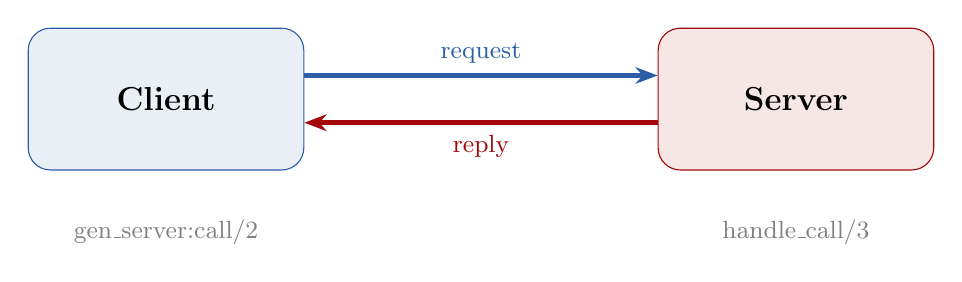
\begin{tikzpicture}
    \node[draw=erlblue, fill=erlblue!10, rounded corners=8pt, minimum width=3.5cm, minimum height=1.8cm, font=\large\bfseries] (client) at (0,0) {Client};
    \node[draw=erlred, fill=erlred!10, rounded corners=8pt, minimum width=3.5cm, minimum height=1.8cm, font=\large\bfseries] (server) at (8,0) {Server};

    \draw[-{Stealth[length=8pt]}, line width=2pt, erlblue]
        ([yshift=3mm]client.east) -- node[above, font=\small] {request} ([yshift=3mm]server.west);
    \draw[-{Stealth[length=8pt]}, line width=2pt, erlred]
        ([yshift=-3mm]server.west) -- node[below, font=\small] {reply} ([yshift=-3mm]client.east);

    \node[below=5mm of client, font=\small\color{gray}] {gen\_server:call/2};
    \node[below=5mm of server, font=\small\color{gray}] {handle\_call/3};
\end{tikzpicture}

\vspace{3cm}

{\large\color{darkgray} 以 counter\_server 为例，从架构到实践}

\vspace{1cm}

{\normalsize\color{gray} Erlang/OTP $\cdot$ Behavior Pattern $\cdot$ Concurrent Programming}

\vfill
{\small\today}
\end{titlepage}

% ---- Table of Contents ----
\newpage
\tableofcontents
\newpage


% ============================================================
% Section 1: Overview
% ============================================================
\section{概述}

\subsection{什么是 gen\_server？}

\texttt{gen\_server} 是 OTP 框架中最核心的行为模式（behavior）之一。它将 Erlang 中常见的客户端--服务器（Client-Server）模式抽象为一个通用的库模块，开发者只需实现回调函数即可获得一个健壮的并发服务器。

\begin{tipbox}[核心思想]
\textbf{gen\_server = Generic Part + Specific Part}

\begin{itemize}[leftmargin=1.5em]
    \item \textbf{Generic Part}（\texttt{gen\_server.erl}）：消息循环、错误处理、超时、sys 集成等通用逻辑
    \item \textbf{Specific Part}（你的回调模块）：\texttt{init/1}、\texttt{handle\_call/3} 等业务逻辑
\end{itemize}
\end{tipbox}

\subsection{gen\_server 提供的能力}

\begin{table}[H]
\centering
\begin{tabular}{@{}ll@{}}
\toprule
\textbf{能力} & \textbf{说明} \\
\midrule
同步调用 (call)    & 客户端发送请求并等待回复 \\
异步调用 (cast)    & 客户端发送请求后立即返回 \\
超时机制           & 支持 call 超时和空闲超时 \\
错误处理           & 自动生成崩溃报告 \\
sys 模块集成       & 支持 trace、statistics、suspend/resume \\
热代码升级         & 通过 code\_change/3 支持运行时升级 \\
进程链接           & 配合 supervisor 实现容错 \\
\bottomrule
\end{tabular}
\caption{gen\_server 提供的能力}
\end{table}

\subsection{OTP 源码中的工作流}

以下直接对应 \texttt{gen\_server.erl} 源码中的注释：

\begin{tcolorbox}[colback=codebg, colframe=codeborder, arc=2mm, boxrule=0.5pt,
                  title={\textbf{gen\_server.erl --- Work Flow}},
                  fonttitle=\bfseries\ttfamily, width=\textwidth]
\small\ttfamily
\begin{tabular}{@{}lcl@{}}
gen\_server module &  & Callback module \\
\textsf{-{}-{}-{}-{}-{}-{}-{}-{}-{}-{}-{}-{}-{}-{}-{}-{}-} & & \textsf{-{}-{}-{}-{}-{}-{}-{}-{}-{}-{}-{}-{}-{}-{}-} \\
gen\_server:start\_link & -{}-{}-{}-{}-> & Module:init/1 \\
gen\_server:stop       & -{}-{}-{}-{}-> & Module:terminate/2 \\
gen\_server:call       & -{}-{}-{}-{}-> & Module:handle\_call/3 \\
gen\_server:cast       & -{}-{}-{}-{}-> & Module:handle\_cast/2 \\
-                     & -{}-{}-{}-{}-> & Module:handle\_info/2 \\
-                     & -{}-{}-{}-{}-> & Module:handle\_continue/2 \\
-                     & -{}-{}-{}-{}-> & Module:code\_change/3 \\
\end{tabular}
\end{tcolorbox}


% ============================================================
% Section 2: Architecture Diagrams
% ============================================================
\section{架构图（通过 Pid）}

使用 \texttt{gen\_server:start\_link(?MODULE, Args, Opts)} 启动，不注册名字，通过返回的 Pid 来调用服务。

\begin{figure}[H]
\centering
\includegraphics[width=\textwidth]{images/gen_server_architecture_pid.pdf}
\caption{架构图（方式一）：通过 PID 引用 --- \texttt{start\_link/3}}
\label{fig:arch-pid}
\end{figure}

\subsection{不注册（使用 PID）}

\begin{lstlisting}[style=erlangstyle]
{ok, Pid} = gen_server:start_link(?MODULE, Args, []).
%% Call by PID: gen_server:call(Pid, Request)
%% Can start multiple instances!
\end{lstlisting}

\subsection{实验演示：本地 PID 场景}

在同一个 Erlang 节点上启动 \texttt{counter\_server}，通过返回的 PID 直接调用。本地进程的 PID 第一位数字始终为 \texttt{0}。

\begin{lstlisting}[style=shellstyle, caption={本地 PID 场景 --- 在 apple 节点上操作}]
[ericksun@ERICKSUN-MC1:src] (main) $ erl -sname apple
Erlang/OTP 26 [erts-14.2.5.12] [source] [64-bit] [smp:12:12]
              [ds:12:12:10] [async-threads:1] [jit] [dtrace]

Eshell V14.2.5.12 (press Ctrl+G to abort, type help(). for help)
(apple@ERICKSUN-MC1)1> {ok, Server}=counter_server:start_link().
[counter] init: count=0, pid=<0.93.0>
[counter] post_init complete
{ok,<0.93.0>}
(apple@ERICKSUN-MC1)2> counter_server:get_count(Server).
0
(apple@ERICKSUN-MC1)3> counter_server:increment(Server).
1
(apple@ERICKSUN-MC1)4> counter_server:increment(Server).
2
(apple@ERICKSUN-MC1)5> counter_server:get_count(Server).
2
\end{lstlisting}

\begin{notebox}[PID 结构]
PID 的格式为 \texttt{<A.B.C>}：
\begin{itemize}[leftmargin=1.5em]
    \item \textbf{A}（第一位）：节点标识。本地节点上始终为 \texttt{0}
    \item \textbf{B}（中间位）：进程在创建节点上的唯一序号，\textbf{无论从哪个节点观察都不变}
    \item \textbf{C}（第三位）：序号溢出后的高位计数器（通常为 \texttt{0}）
\end{itemize}
上例中 \texttt{<0.93.0>} 表示：本地节点（\texttt{0}）、进程序号 \texttt{93}、高位 \texttt{0}。
\end{notebox}

\subsection{实验演示：分布式 PID 场景（跨节点访问）}

在另一个 Erlang 节点（\texttt{pear}）上，通过 PID 远程访问 \texttt{apple} 节点上的 \texttt{counter\_server}。关键特性：\textbf{PID 中间的数字在远程节点上看到的不变}，但第一位数字从 \texttt{0} 变为非零值。

\begin{lstlisting}[style=shellstyle, caption={分布式 PID 场景 --- 从 pear 节点远程访问 apple 节点}]
[ericksun@ERICKSUN-MC1:src] (main) $ erl -sname pear
Erlang/OTP 26 [erts-14.2.5.12] [source] [64-bit] [smp:12:12]
              [ds:12:12:10] [async-threads:1] [jit] [dtrace]

Eshell V14.2.5.12 (press Ctrl+G to abort, type help(). for help)
(pear@ERICKSUN-MC1)1> net_adm:ping('apple@ERICKSUN-MC1').
pong
(pear@ERICKSUN-MC1)2> nodes().
['apple@ERICKSUN-MC1']
(pear@ERICKSUN-MC1)3> [Server | _] = lists:filter(
    fun(P) ->
        case string:tokens(pid_to_list(P), ".<>") of
            [_, M, _] -> list_to_integer(M) =:= 93;
            _ -> false
        end
    end,
    rpc:call('apple@ERICKSUN-MC1', erlang, processes, [])).
[<10244.93.0>]
(pear@ERICKSUN-MC1)4> Server.
<10244.93.0>
(pear@ERICKSUN-MC1)5> counter_server:get_count(Server).
2
(pear@ERICKSUN-MC1)6> counter_server:increment(Server).
3
(pear@ERICKSUN-MC1)7> counter_server:decrement(Server).
2
(pear@ERICKSUN-MC1)8> counter_server:get_count(Server).
2
\end{lstlisting}

\begin{tipbox}[分布式 PID 的关键观察]
\begin{itemize}[leftmargin=1.5em]
    \item 在 \texttt{apple} 节点上，PID 显示为 \texttt{<0.93.0>}（第一位为 \texttt{0}，表示本地）
    \item 在 \texttt{pear} 节点上，同一进程的 PID 显示为 \texttt{<10244.93.0>}（第一位为 \texttt{10244}，表示远程节点在本地连接表中的编号）
    \item \textbf{中间数字 93 始终不变}，这是进程在其创建节点上的唯一标识
    \item Erlang 运行时根据 PID 中的节点信息自动路由消息，\textbf{调用方式与本地完全相同}
\end{itemize}
\end{tipbox}


\section{架构图（通过名字）}

使用 \texttt{gen\_server:start\_link(ServerName, ?MODULE, Args, Opts)} 启动，将进程注册到名字表，Client 通过名字调用服务。

\begin{figure}[H]
\centering
\includegraphics[width=\textwidth]{images/gen_server_architecture_named.pdf}
\caption{架构图（方式二）：通过注册名字引用 --- \texttt{start\_link/4}}
\label{fig:arch-named}
\end{figure}

gen\_server 支持多种进程注册方式：

\subsection{本地注册}

\begin{lstlisting}[style=erlangstyle]
gen_server:start_link({local, counter}, ?MODULE, Args, []).
%% Call by name: gen_server:call(counter, Request)
%% Only visible on current node
\end{lstlisting}

\paragraph{实验演示：本地注册在集群中互不影响}

本地注册（\texttt{\{local, Name\}}）的名字仅在当前节点可见。在集群中，\textbf{每个节点可以各自注册同名进程，互不影响}。

\textbf{节点 apple} --- 启动并注册 \texttt{counter\_local}：

\begin{lstlisting}[style=shellstyle, caption={apple 节点 --- 本地注册 counter\_local}]
(apple@ERICKSUN-MC1)1> named_counter:start_link_local().
[named_counter] init: count=0, pid=<0.93.0>,
    local_name=counter_local, global_name=undefined
{ok,<0.93.0>}
(apple@ERICKSUN-MC1)2> whereis(counter_local).
<0.93.0>
(apple@ERICKSUN-MC1)3> named_counter:get_count(counter_local).
0
(apple@ERICKSUN-MC1)4> named_counter:increment(counter_local).
1
(apple@ERICKSUN-MC1)5> named_counter:increment(counter_local).
2
(apple@ERICKSUN-MC1)6> named_counter:get_count(counter_local).
2
\end{lstlisting}

\textbf{节点 pear} --- 连接到 apple 后，\texttt{counter\_local} 在本节点不可见，可以独立注册同名进程，也可以通过 \texttt{rpc} 以名字调用远程节点的函数：

\begin{lstlisting}[style=shellstyle, caption={pear 节点 --- 独立注册同名 counter\_local 并通过 rpc 调用远程}]
(pear@ERICKSUN-MC1)1> net_adm:ping('apple@ERICKSUN-MC1').
pong
(pear@ERICKSUN-MC1)2> whereis(counter_local).
undefined
(pear@ERICKSUN-MC1)3> nodes().
['apple@ERICKSUN-MC1']
(pear@ERICKSUN-MC1)4> named_counter:start_link_local().
[named_counter] init: count=0, pid=<0.102.0>,
    local_name=counter_local, global_name=undefined
{ok,<0.102.0>}
(pear@ERICKSUN-MC1)5> named_counter:increment(counter_local).
1
(pear@ERICKSUN-MC1)6> named_counter:increment(counter_local).
2
(pear@ERICKSUN-MC1)7> named_counter:get_count(counter_local).
2
(pear@ERICKSUN-MC1)8> rpc:call('apple@ERICKSUN-MC1',
    erlang, whereis, [counter_local]).
<10244.93.0>
(pear@ERICKSUN-MC1)9> rpc:call('pear@ERICKSUN-MC1',
    erlang, whereis, [counter_local]).
<0.102.0>
(pear@ERICKSUN-MC1)10> rpc:call('apple@ERICKSUN-MC1',
    named_counter, increment, [counter_local]).
3
(pear@ERICKSUN-MC1)11> rpc:call('apple@ERICKSUN-MC1',
    named_counter, increment, [counter_local]).
4
(pear@ERICKSUN-MC1)12> rpc:call('apple@ERICKSUN-MC1',
    named_counter, get_count, [counter_local]).
4
\end{lstlisting}

\begin{tipbox}[本地注册的关键特性]
\begin{itemize}[leftmargin=1.5em]
    \item \texttt{whereis(counter\_local)} 在 pear 节点上返回 \texttt{undefined}，说明 apple 节点的本地注册名在 pear 上\textbf{不可见}
    \item pear 节点可以独立注册同名的 \texttt{counter\_local}，两个节点上的进程\textbf{完全独立}，各自维护自己的状态
    \item 这正是 \texttt{\{local, Name\}} 的语义：名字的作用域仅限于当前 Erlang 节点
    \item 通过 \texttt{rpc:call/4} 可以以本地注册名调用远程节点上的函数。\texttt{rpc:call('apple@...', named\_counter, increment, [counter\_local])} 会在 apple 节点上执行，操作的是 apple 上的 \texttt{counter\_local} 进程（计数从 2 增加到 4），而 pear 本地的 \texttt{counter\_local} 不受影响
    \item \texttt{rpc:call} 查询 \texttt{whereis} 可以看到：apple 上的 PID 为 \texttt{<10244.93.0>}（远程视角），pear 上的 PID 为 \texttt{<0.102.0>}（本地视角），两者是完全不同的进程
\end{itemize}
\end{tipbox}

\subsection{全局注册}

\begin{lstlisting}[style=erlangstyle]
gen_server:start_link({global, counter}, ?MODULE, Args, []).
%% Call: gen_server:call({global, counter}, Request)
%% Visible on all connected nodes (distributed)
\end{lstlisting}

\paragraph{实验演示：全局注册在集群中唯一可见}

全局注册（\texttt{\{global, GlobalName\}}）的名字通过 \texttt{global} 模块在整个集群中维护，\textbf{所有连接的节点都能看到并直接使用}。与本地注册不同，全局名字在集群中只能有一个。

\textbf{节点 apple} --- 启动并全局注册 \texttt{counter\_global}：

\begin{lstlisting}[style=shellstyle, caption={apple 节点 --- 全局注册 counter\_global}]
[ericksun@ERICKSUN-MC1:src] (main) $ erl -sname apple
Erlang/OTP 26 [erts-14.2.5.12] [source] [64-bit] [smp:12:12]
              [ds:12:12:10] [async-threads:1] [jit] [dtrace]

Eshell V14.2.5.12 (press Ctrl+G to abort, type help(). for help)
(apple@ERICKSUN-MC1)1> global_counter:start_link_global().
[global_counter] init: count=0, pid=<0.93.0>,
    global_name=counter_global
{ok,<0.93.0>}
(apple@ERICKSUN-MC1)2> global:registered_names().
[counter_global]
(apple@ERICKSUN-MC1)3> global_counter:increment({global,
    counter_global}).
1
(apple@ERICKSUN-MC1)4> global_counter:increment({global,
    counter_global}).
2
(apple@ERICKSUN-MC1)5> global_counter:get_count({global,
    counter_global}).
3
\end{lstlisting}

\textbf{节点 pear} --- 连接到 apple 后，\texttt{counter\_global} 在 pear 节点上\textbf{直接可见}，无需 \texttt{rpc}，直接通过 \texttt{\{global, counter\_global\}} 即可调用：

\begin{lstlisting}[style=shellstyle, caption={pear 节点 --- 直接通过全局名字访问 apple 上的 counter\_global}]
[ericksun@ERICKSUN-MC1:src] (main) $ erl -sname pear
Erlang/OTP 26 [erts-14.2.5.12] [source] [64-bit] [smp:12:12]
              [ds:12:12:10] [async-threads:1] [jit] [dtrace]

Eshell V14.2.5.12 (press Ctrl+G to abort, type help(). for help)
(pear@ERICKSUN-MC1)1> net_adm:ping('apple@ERICKSUN-MC1').
pong
(pear@ERICKSUN-MC1)2> nodes().
['apple@ERICKSUN-MC1']
(pear@ERICKSUN-MC1)3> global:registered_names().
[counter_global]
(pear@ERICKSUN-MC1)4> global_counter:increment({global,
    counter_global}).
3
\end{lstlisting}

\begin{tipbox}[全局注册的关键特性]
\begin{itemize}[leftmargin=1.5em]
    \item \texttt{global:registered\_names()} 在 pear 节点上也返回 \texttt{[counter\_global]}，说明全局名字在\textbf{整个集群中可见}
    \item pear 节点无需 \texttt{rpc:call}，直接使用 \texttt{global\_counter:increment(\{global, counter\_global\})} 即可操作 apple 上的进程
    \item apple 节点上 increment 两次后 \texttt{get\_count} 返回 \texttt{3}（因为两个节点操作的是\textbf{同一个服务}），pear 节点 increment 后返回 \texttt{3}，状态在集群中\textbf{完全一致}
    \item 全局名字在集群中\textbf{唯一}：如果 pear 节点也尝试 \texttt{start\_link\_global()}，会因为名字已被占用而返回 \texttt{\{error, \{already\_started, Pid\}\}}
    \item 这正是 \texttt{\{global, Name\}} 与 \texttt{\{local, Name\}} 的核心区别：全局注册提供集群级别的单例语义
\end{itemize}
\end{tipbox}

\subsection{server\_ref() 完整类型}

\begin{table}[H]
\centering
\begin{tabular}{@{}ll@{}}
\toprule
\textbf{类型} & \textbf{说明} \\
\midrule
\texttt{pid()} & 直接 PID 引用 \\
\texttt{atom()} & 本地注册名 \\
\texttt{\{Name, Node\}} & 远程节点的本地注册名 \\
\texttt{\{global, GlobalName\}} & 全局注册名 \\
\texttt{\{via, RegMod, ViaName\}} & 自定义注册模块 \\
\bottomrule
\end{tabular}
\caption{server\_ref() 类型一览}
\end{table}




% ============================================================
% Section 3: Example — counter_server
% ============================================================
\section{实例：counter\_server}

\begin{notebox}[源码文件]
\texttt{src/counter\_server.erl}
\end{notebox}

以一个计数器服务器为例，完整展示 gen\_server 的用法。

\subsection{模块声明}

\begin{lstlisting}[style=erlangstyle, caption={模块声明与行为模式}]
-module(counter_server).
-behaviour(gen_server).

%% Client API
-export([start_link/0, start_link/1, start/0, start/1]).
-export([increment/1, decrement/1, get_count/1, reset/1]).
-export([slow_operation/2, crash/1]).

%% gen_server callbacks
-export([init/1, handle_call/3, handle_cast/2,
         handle_info/2, handle_continue/2,
         terminate/2, code_change/3, format_status/2]).
\end{lstlisting}

\subsection{启动函数}

\begin{lstlisting}[style=erlangstyle, caption={启动函数 --- start\_link 与 start}]
start_link() ->
    gen_server:start_link(?MODULE, 0, []).
%%                        ^^^^^^  ^  ^^
%%                        Module  Arg Options

start_link(InitCount) ->
    gen_server:start_link(?MODULE, InitCount, []).

start() ->
    gen_server:start(?MODULE, 0, []).

start(InitCount) ->
    gen_server:start(?MODULE, InitCount, []).
\end{lstlisting}

\begin{tipbox}[start\_link vs start]
\begin{itemize}[leftmargin=1.5em]
    \item \texttt{start\_link}：与调用者进程链接，一方崩溃另一方也会收到通知。生产环境配合 supervisor 使用。
    \item \texttt{start}：不链接，独立生命周期。适合开发测试。
\end{itemize}
\end{tipbox}

\subsection{客户端 API}

\begin{lstlisting}[style=erlangstyle, caption={客户端 API --- 对 gen\_server 调用的封装}]
increment(Server) ->
    gen_server:call(Server, increment).     %% sync

decrement(Server) ->
    gen_server:call(Server, decrement).     %% sync

get_count(Server) ->
    gen_server:call(Server, get_count).     %% sync

reset(Server) ->
    gen_server:cast(Server, reset).         %% async

slow_operation(Server, Duration) ->
    gen_server:call(Server, {slow_op, Duration}).

crash(Server) ->
    gen_server:cast(Server, crash).
\end{lstlisting}

\begin{warnbox}[注意]
客户端 API 是\textbf{薄封装}（thin wrapper），它们运行在\textbf{调用者进程}中，而非 gen\_server 进程中。
\end{warnbox}

\subsection{init/1 --- 初始化}

\begin{lstlisting}[style=erlangstyle, caption={init/1 --- 初始化回调}]
init(InitCount) when is_integer(InitCount) ->
    process_flag(trap_exit, true),
    io:format("[counter] init: count=~p, pid=~p~n",
              [InitCount, self()]),
    {ok, #{count => InitCount, history => []},
     {continue, post_init}};
init(_) ->
    {stop, {error, bad_init_arg}}.
\end{lstlisting}

要点：
\begin{itemize}[leftmargin=2em]
    \item State 使用 Map：\texttt{\#\{count => 0, history => []\}}
    \item \texttt{process\_flag(trap\_exit, true)}：捕获 EXIT 信号，使 \texttt{terminate/2} 能被调用
    \item \texttt{\{continue, post\_init\}}：init 返回后立即触发 \texttt{handle\_continue/2}
\end{itemize}

\subsection{handle\_continue/2 --- 延续处理}

\begin{lstlisting}[style=erlangstyle, caption={handle\_continue/2 --- 初始化后的延续}]
handle_continue(post_init, State) ->
    io:format("[counter] post_init complete~n"),
    {noreply, State}.
\end{lstlisting}

\begin{tipbox}[为什么用 handle\_continue？]
\texttt{init/1} 应该尽快返回（因为调用者在等待 \texttt{\{ok, Pid\}}）。耗时的初始化工作可以放到 \texttt{handle\_continue/2} 中异步完成。
\end{tipbox}

\subsection{handle\_call/3 --- 同步请求}

\begin{lstlisting}[style=erlangstyle, caption={handle\_call/3 --- 处理同步请求}]
handle_call(increment, _From, #{count := C} = State) ->
    NewCount = C + 1,
    {reply, NewCount, State#{count := NewCount,
        history := [{increment, NewCount} |
                    maps:get(history, State)]}};

handle_call(decrement, _From, #{count := C} = State) ->
    NewCount = C - 1,
    {reply, NewCount, State#{count := NewCount,
        history := [{decrement, NewCount} |
                    maps:get(history, State)]}};

handle_call(get_count, _From, #{count := C} = State) ->
    {reply, C, State};

handle_call({slow_op, Duration}, _From, State) ->
    timer:sleep(Duration),
    {reply, {ok, done_after, Duration}, State};

handle_call(_Request, _From, State) ->
    {reply, {error, unknown_request}, State}.
\end{lstlisting}

\subsection{handle\_cast/2 --- 异步请求}

\begin{lstlisting}[style=erlangstyle, caption={handle\_cast/2 --- 处理异步请求}]
handle_cast(reset, State) ->
    io:format("[counter] reset to 0~n"),
    {noreply, State#{count := 0, history := []}};

handle_cast(crash, _State) ->
    error(deliberate_crash);

handle_cast(_Msg, State) ->
    {noreply, State}.
\end{lstlisting}

\subsection{handle\_info/2 --- 其他消息}

\begin{lstlisting}[style=erlangstyle, caption={handle\_info/2 --- 处理非 call/cast 消息}]
handle_info(timeout, State) ->
    io:format("[counter] timeout fired~n"),
    {noreply, State};

handle_info({custom_msg, Payload}, State) ->
    io:format("[counter] received custom_msg: ~p~n", [Payload]),
    {noreply, State};

handle_info({'EXIT', Pid, Reason}, State) ->
    io:format("[counter] linked process ~p exited: ~p~n",
              [Pid, Reason]),
    {noreply, State};

handle_info(Info, State) ->
    io:format("[counter] unexpected info: ~p~n", [Info]),
    {noreply, State}.
\end{lstlisting}

\subsection{terminate/2 --- 终止清理}

\begin{lstlisting}[style=erlangstyle, caption={terminate/2 --- 进程终止时的清理}]
terminate(Reason, #{count := C}) ->
    io:format("[counter] terminating: reason=~p, "
              "final_count=~p~n", [Reason, C]),
    ok.
\end{lstlisting}

\subsection{format\_status/2 --- 自定义状态显示}

\begin{lstlisting}[style=erlangstyle, caption={format\_status/2 --- 自定义 sys:get\_status 输出}]
format_status(_Opt, [_PDict, #{count := C, history := H}]) ->
    [{data, [{"State",
              #{count => C,
                history_length => length(H)}}]}].
\end{lstlisting}

\begin{tipbox}[安全提示]
\texttt{format\_status/2} 可用于隐藏敏感信息（如密码、token），使其不出现在崩溃日志和 \texttt{sys:get\_status/1} 输出中。
\end{tipbox}


% ============================================================
% Section 4: Message Flow
% ============================================================
\section{消息流转}

\begin{figure}[H]
\centering
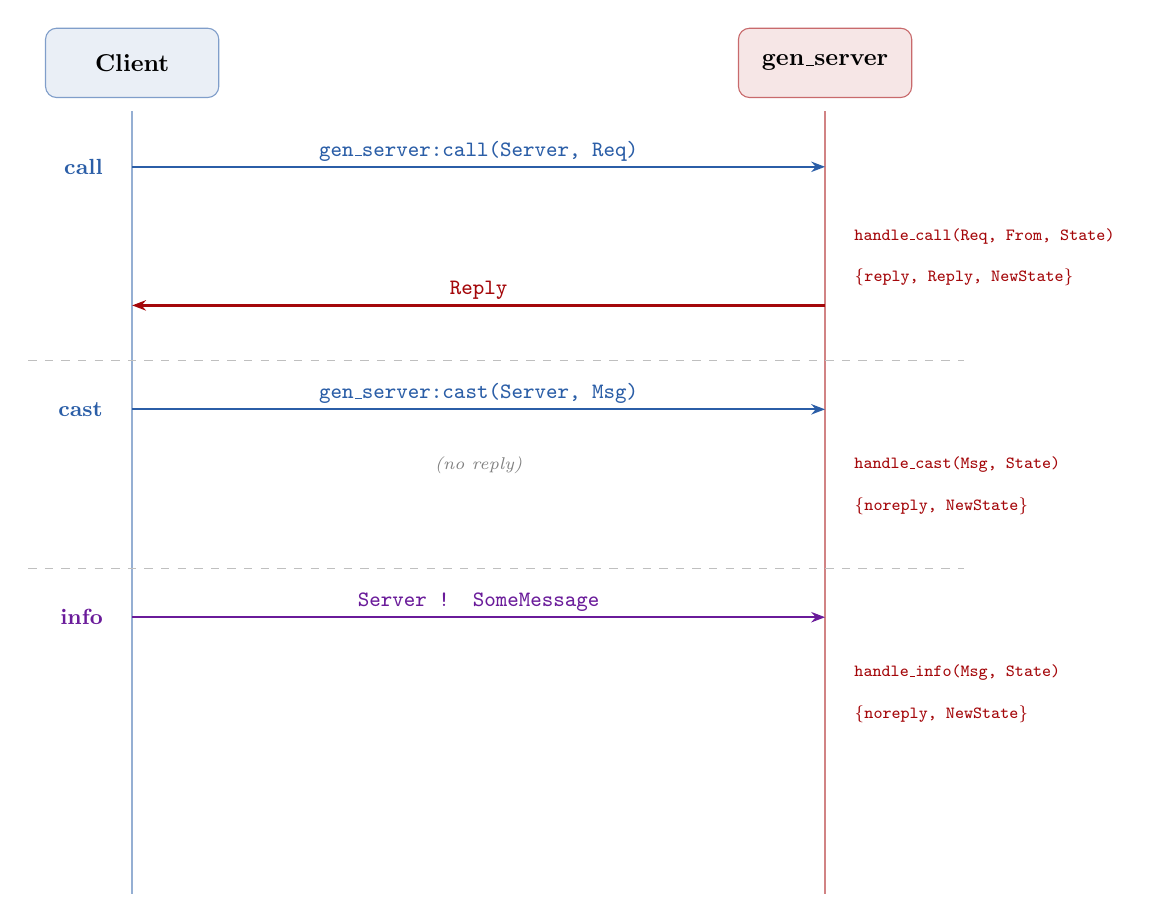
\begin{tikzpicture}[scale=0.88, every node/.style={scale=0.88},
    actor/.style={draw, rounded corners=4pt, fill=#1!10, draw=#1!60,
                  minimum width=2.5cm, minimum height=1cm, font=\bfseries},
    msg/.style={-{Stealth[length=5pt]}, thick, #1},
    lbl/.style={font=\small\ttfamily, fill=white, inner sep=2pt},
]
    \node[actor=erlblue] (client) at (0, 0) {Client};
    \node[actor=erlred] (server) at (10, 0) {gen\_server};

    \draw[thick, erlblue!50] (0, -0.7) -- (0, -12);
    \draw[thick, erlred!50] (10, -0.7) -- (10, -12);

    % === call ===
    \node[font=\small\bfseries\color{erlblue}, anchor=east] at (-0.3, -1.5) {call};
    \draw[msg=erlblue] (0, -1.5) -- node[lbl, above] {gen\_server:call(Server, Req)} (10, -1.5);
    \node[font=\scriptsize\ttfamily, anchor=west, text=erlred] at (10.3, -2.5) {handle\_call(Req, From, State)};
    \node[font=\scriptsize\ttfamily, anchor=west, text=erlred] at (10.3, -3.1) {\{reply, Reply, NewState\}};
    \draw[msg=erlred] (10, -3.5) -- node[lbl, above] {Reply} (0, -3.5);

    % === cast ===
    \node[font=\small\bfseries\color{erlblue}, anchor=east] at (-0.3, -5) {cast};
    \draw[msg=erlblue] (0, -5) -- node[lbl, above] {gen\_server:cast(Server, Msg)} (10, -5);
    \node[font=\scriptsize\ttfamily, anchor=west, text=erlred] at (10.3, -5.8) {handle\_cast(Msg, State)};
    \node[font=\scriptsize\ttfamily, anchor=west, text=erlred] at (10.3, -6.4) {\{noreply, NewState\}};
    \node[font=\scriptsize\itshape\color{gray}] at (5, -5.8) {(no reply)};

    % === info ===
    \node[font=\small\bfseries\color{erlpurple}, anchor=east] at (-0.3, -8) {info};
    \draw[msg=erlpurple] (0, -8) -- node[lbl, above] {Server ! SomeMessage} (10, -8);
    \node[font=\scriptsize\ttfamily, anchor=west, text=erlred] at (10.3, -8.8) {handle\_info(Msg, State)};
    \node[font=\scriptsize\ttfamily, anchor=west, text=erlred] at (10.3, -9.4) {\{noreply, NewState\}};

    % Dashed separators
    \draw[dashed, gray!50] (-1.5, -4.3) -- (12, -4.3);
    \draw[dashed, gray!50] (-1.5, -7.3) -- (12, -7.3);
\end{tikzpicture}
\caption{gen\_server 三种消息类型的流转过程}
\label{fig:message-flow}
\end{figure}

\subsection{常见陷阱}

\begin{itemize}[leftmargin=2em]
    \item \textbf{Shell 中使用 start\_link}：Shell 进程与 gen\_server 链接，gen\_server 崩溃会导致 Shell 也崩溃。开发测试时建议使用 \texttt{start/0}
    \item \textbf{handle\_call 中调用自己}：\texttt{gen\_server:call(self(), Req)} 会死锁，因为 gen\_server 是单进程的，处理消息时无法再接收新消息
    \item \textbf{call 超时后的残留消息}：超时时客户端崩溃，但服务器继续运行并可能稍后发送回复，残留消息会留在调用者的消息队列中
    \item \textbf{handle\_call 中的长时间操作}：gen\_server 顺序处理消息，长时间操作会阻塞所有其他请求。可用 \texttt{cast} + 异步通知、spawn 子进程、或 \texttt{gen\_server:reply/2} 解决
\end{itemize}


% ============================================================
% Section 5: Callback Return Values
% ============================================================
\section{回调函数返回值}

\subsection{init/1}

\begin{lstlisting}[style=erlangstyle]
init(Args) ->
    {ok, State}                  %% Normal start
  | {ok, State, Timeout}         %% Start with timeout
  | {ok, State, hibernate}       %% Start and hibernate
  | {ok, State, {continue, Info}} %% Start with continuation
  | {stop, Reason}               %% Start failed
  | ignore.                      %% Ignore start
\end{lstlisting}

\subsection{handle\_call/3}

\begin{lstlisting}[style=erlangstyle]
handle_call(Request, From, State) ->
    {reply, Reply, NewState}              %% Reply and continue
  | {reply, Reply, NewState, Timeout}     %% Reply, set timeout
  | {reply, Reply, NewState, hibernate}   %% Reply, hibernate
  | {reply, Reply, NewState, {continue, Info}} %% Reply, continue
  | {noreply, NewState}                   %% No reply (manual)
  | {noreply, NewState, Timeout}
  | {stop, Reason, Reply, NewState}       %% Reply then stop
  | {stop, Reason, NewState}.             %% Stop (no reply)
\end{lstlisting}

\subsection{handle\_cast/2}

\begin{lstlisting}[style=erlangstyle]
handle_cast(Msg, State) ->
    {noreply, NewState}
  | {noreply, NewState, Timeout}
  | {noreply, NewState, hibernate}
  | {noreply, NewState, {continue, Info}}
  | {stop, Reason, NewState}.
\end{lstlisting}

\subsection{handle\_info/2}

返回值与 \texttt{handle\_cast/2} 相同。

\subsection{terminate/2}

\begin{lstlisting}[style=erlangstyle]
terminate(Reason, State) ->
    ok.  %% Return value is ignored
\end{lstlisting}

\begin{warnbox}[注意]
\texttt{terminate/2} 只在以下情况被调用：
\begin{itemize}
    \item 回调函数返回 \texttt{\{stop, ...\}}
    \item 进程收到 EXIT 信号且设置了 \texttt{process\_flag(trap\_exit, true)}
    \item \texttt{gen\_server:stop/1,3} 被调用
\end{itemize}
\end{warnbox}




\end{document}
